\documentclass[11pt,a4paper]{article}

\usepackage{epsfig,latexsym,amsbsy,amssymb,amsmath,color, url, natbib, booktabs, multirow}
\usepackage{colortbl}
\usepackage{longtable}
\usepackage{natbib}
\usepackage{algorithm,algorithmic}
\oddsidemargin  0.0in
\evensidemargin 0.0in
\textwidth      6.5in
\headheight     0.0in
\topmargin     -1.0in
\textheight=10.0in
\parindent=0in 


\newcommand{\rks}{{\sc rks}}
\renewcommand{\t}{\vecS{\tau}}
\newcommand{\w}{\vec{w}}
\newcommand{\dw}{d\vec{w}}
\newcommand{\dt}{d\t}
\renewcommand{\t}{\vecS{\tau}}
\newcommand{\x}{\vec{x}}
\newcommand{\y}{\vec{y}}
\newcommand{\real}{\mathbb{R}\text{e}}
\newcommand{\phiw}{\phi_{\w}}
\newcommand{\vphi}{\vecS{\phi}}
\newcommand{\vphiw}{\vphi_{\w}}
\newcommand{\sigmaw}{\sigma_w}
% genereal purpose macros here
\newcommand{\marg}{\marginpar}
\newcommand{\commentOut}[1]{} 
\newcommand{\add}[1]{\textcolor{red}{#1}} % To highligh modified text
\newcommand{\red}[1]{{\color{red}{#1}}}
\newcommand{\fix}[1]{\red{(#1)} \marginpar{\red{FIX}}}
\newcommand{\todo}[1]{{\fix{TODO: #1}}}


% abbreviations
\newcommand{\etal}{et al.\xspace}
\newcommand{\ie}{i.e.\xspace}
\newcommand{\eg}{e.g.\xspace}
\newcommand{\Ie}{I.e.\xspace}



% Matrices and vectors 
\newcommand{\mat}[1]{\mathbf{#1}}
\renewcommand{\vec}[1]{ \mathbf{#1} } % math bold
\newcommand{\vecS}[1]{\boldsymbol{ #1 }  } % this for boldsymbols
\newcommand{\vecentry}[2]{{\mathrm #1_{#2}}}
\newcommand{\matentry}[3]{{\mathrm #1_{#2,#3}}}
\newcommand{\matcol}[2]{\mat{#1}_{\cdot,#2}}
\newcommand{\matrow}[2]{\mat{#1}_{#2,\cdot}}

 % Matrices and vectors here
 \newcommand{\A}{\mat{A}}
\newcommand{\B}{\mat{B}}
\newcommand{\C}{\mat{C}}
\newcommand{\D}{\mat{D}}
\newcommand{\E}{\mat{E}}
\newcommand{\F}{\mat{F}}
\newcommand{\G}{\mat{G}}
\newcommand{\I}{\mat{I}}
\newcommand{\K}{\mat{K}}
\renewcommand{\L}{\mat{L}}
\newcommand{\Q}{\mat{Q}}
\newcommand{\X}{\mat{X}}
\newcommand{\W}{\mat{W}}
\newcommand{\Y}{\mat{Y}}
\newcommand{\Z}{\mat{Z}}


 % Vectorial greek letters
 \newcommand{\vecalpha}{\vecS{\alpha}}
 \newcommand{\vecphi}{\vecS{\phi}}
 \newcommand{\veceta}{\vecS{\eta}}
  
 
% caligraphic alphabet
\newcommand{\calA}{\mathcal{A}}
\newcommand{\calC}{\mathcal{C}}
\newcommand{\calD}{\mathcal{D}} 
\newcommand{\calL}{\mathcal{L}}
\newcommand{\calM}{\mathcal{M}}
\newcommand{\calT}{\mathcal{T}}
\newcommand{\calU}{\mathcal{U}}
\newcommand{\calX}{\mathcal{X}}
\newcommand{\calF}{\mathcal{F}}
\newcommand{\calE}{\mathcal{E}}
\newcommand{\calI}{\mathcal{I}}
\newcommand{\calS}{\mathcal{S}}
\newcommand{\calY}{\mathcal{Y}}
\newcommand{\calO}{\mathcal{O}}
\newcommand{\calQ}{\mathcal{Q}}
\newcommand{\calR}{\mathcal{R}}
\newcommand{\calV}{\mathcal{V}}

% Tilde Alphabet
\newcommand{\tildeN}{\tilde{N}}

% blackboard alphabet 
\newcommand{\setR}{\mathbb{R}}
\newcommand{\setE}{\mathbb{E}}
\newcommand{\setV}{\mathbb{V}}
\newcommand{\setI}{\mathbb{I}}
\newcommand{\setX}{\mathbb{X}}
\newcommand{\setT}{\mathbb{T}}
\newcommand{\setU}{\mathbb{U}}



% Useful math operators
\newcommand{\Sum}{{\displaystyle \sum}}
\DeclareMathOperator{\vect}{vec}
\DeclareMathOperator{\diag}{diag}
\DeclareMathOperator*{\argmax}{argmax}                 
\DeclareMathOperator*{\argmin}{argmin}                 
\providecommand{\abs}[1]{\lvert#1\rvert}
\providecommand{\norm}[1]{\lVert#1\rVert}
\newcommand{\notp}[1]{\stackrel{\neg}{#1}} % symbol for not present


% matrix products
\newcommand{\kron}{\otimes}
\newcommand{\hada}{\odot}

% statistics
\newcommand{\expectation}{\mathbb{E}}
\newcommand{\Eb}[1]{\left\langle #1 \right\rangle} % Expectation in angle brackets
\newcommand{\variance}{\mathbb{V}}
\newcommand{\covariance}{\mathbb{C}\text{ov}}
\newcommand{\Normal}{\mathcal{N}}  
\newcommand{\avg}[1]{\overline{#1}}


% GP things
\newcommand{\GP}{\mathcal{GP}}
\newcommand{\kernel}{\kappa}

% Other maths
\newcommand{\deriv}[2]{\frac{\partial{#1}}{\partial{#2}}}
\newcommand{\fullderiv}[2]{\frac{d{#1}}{d{#2}}}
\newcommand{\secondderiv}[2]{\frac{\partial^{2}{#1}}{\partial{#2^{2}}}}
\newcommand{\derivtwo}[2]{\frac{\partial^{2}{#1}}{\partial{#2}}}
\newcommand{\gradient}{\nabla}
\newcommand{\hessian}{\nabla\nabla}
\newcommand{\hessentry}[2]{\frac{\partial^{2}}{\partial{#1}\partial{#2}}}
\newcommand{\trace}{\mbox{ \rm tr }}
\renewcommand{\det}[1]{\left\lvert#1\right\rvert}
\newcommand{\defeq}{\stackrel{\text{\tiny def}}{=}}
\newcommand{\idx}{\mathcal{I}}
\newcommand{\T}{\text{T}}
\newcommand{\mth}{\mathrm{th}} 


\newcommand{\bigO}{\calO}



\newcommand{\kl}[2]{\mathrm{KL}(#1 \lVert #2)}

















\title{Understanding Random Kitchen Sinks}
\author{Edwin V.~Bonilla}
\begin{document}
\maketitle
In this paper we make sense of the Random Kitchen Sinks (\rks) method \fix{add ref}, which 
approximates a kernel using a finite set of random features.
%
\section{Approximations for Stationary Kernels}
The main starting point is Bochner's theorem regarding stationary processes, which in turn 
yields Wiener-Khintchine's theorem on the Fourier duality of the covariance function of the process
and its spectral density:
\begin{align}
	\kernel(\t) &= \int f(\w) e^{2 \pi i \w^T \t } \dw \text{,} \\
	\label{eq:ft}
			 f(\w) &= \int \kernel(\t) e^{- 2 \pi i \w^T \t } \dt \text{.}
\end{align}
Ali Rahimi's main insight is that we can approximate the above kernel by explicitly constructing 
``suitable" features and (Monte Carlo) averaging over samples from $f(\w)$: 
\begin{align}
	\kernel(\x, \y) = \kernel(\x-\y) = \kernel(\t) &= \expectation_{\w}[\vphiw(\x)^T \vphiw(\y)] \\
	\label{eq:mcapprox}
	& \approx \frac{1}{D} \sum_{i=1}^D {\phiw}_i(\x) {\phiw}_i(\y)
\end{align}
\subsection{Features}
As the kernel 
 $\kernel(\x,\y) = \kernel(\x-\y) = \kernel(\t)$ is  real, and the density $f(\w)$ is real, then we only care about 
 the real part:
\begin{align}
  \label{eq:realfeat}
   \Re\{e^{2 \pi i \w^T \t }\} = \cos(2 \pi  \w^T \t) = \cos(2 \pi \w^T(\x - \y))
\end{align} 
If we use features of the form: 
\begin{align}
	\vphiw(\x) = [\cos( 2 \pi \vec{w}^T  \x) , \sin( 2 \pi \vec{w}^T \x) ]^T \text{,}
\end{align}
Then we have that:
\begin{align}
	\vphiw(\x)^T \vphiw(\y) &=  \cos( 2 \pi \vec{w}^T  \x)  \cos( 2 \pi \vec{w}^T  \y) + \sin( 2 \pi \vec{w}^T \x) \sin( 2 \pi \vec{w}^T \y)\\
	& = \cos(2 \pi \w^T (\x - \y)) \text{,}
\end{align}
where we have obtained the features of the type required by Equation \eqref{eq:realfeat}. Now, 
we can define our vector of features as:
\begin{align}
	\vphiw(\x) = \frac{1}{\sqrt{D}} [ \cos(2 \pi \w_1^T \x), \ldots, \cos(2 \pi \w_D^T \x),
										\ldots \sin(2 \pi \w_1^T \x), \ldots \sin(2 \pi \w_D^T \x)]^T 
\end{align}
so that when computing the dot product $\vphiw(\x)^T \vphiw(\y)$ we obtain the approximation 
in Equation \eqref{eq:mcapprox}.
%
\subsection{Density for the Weights}
A question remains on what density should the weights be sampled from. This, of course, depends on the kernel. 
For the isotropic squared exponential covariance function we have:
\begin{align}
	\kernel(\t) = \exp(- \frac{1}{2 \ell^2} \norm{\t}^2 ) \text{,}
\end{align}
where $\t$ lies in the original input dimensional space $\Re^d$. Having this, it is a matter of computing 
the Fourier transform in Equation \eqref{eq:ft}.
We will derive the density for the weights corresponding to this covariance function in 1-dimension as 
the Fourier transform of decomposable functions is simply the product of the individual Fourier transforms. \\ \\

The Fourier transform of $\kernel(\tau) = \exp(- \frac{1}{2 \ell^2} \tau^2) $ is given by:
\begin{align}
	f(w) & = \sqrt{2 \pi \ell^2} \exp( - 2 \pi^2 \ell^2 w^2) \\
	&= \sqrt{2 \pi \ell^2}  \exp\left( - \frac{1}{2} w^2 \frac{1}{(2 \pi \ell)^{-2}} \right) \\
	&= \sqrt{2 \pi \ell^2} \Normal(w;0, (2 \pi \ell)^{-2}) \frac{\sqrt{2 \pi}}{2 \pi \ell} \quad \text{ \tiny Made the exponential 
	a normalized Gaussian} \\
	&= \frac{1}{2\pi \ell} \Normal(w; 0, 1) \\
	& = \sigmaw \Normal(w; 0, 1) \text{,}
\end{align}
where $\sigmaw^2 = {1}/{(2\pi \ell)^2}$ is the variance of the Gaussian from which the weights are to be sampled.
This is the optimal setting when the length-scale of the GP is known. 
For $D$ new features and d input dimensions, we simply sample $D \times d$ standard Gaussian variables and
 multiply them by $\sigmaw$, which becomes a parameter of the features, as we may want to optimize 
 this when the true length-scale of the process is unknown.
 %
 \subsection{Other Conventions for the Fourier Transforms}
 Ali Rahimi, in fact, follows a different convention for the Fourier and Inverse Fourier Transforms:
 \begin{align}
	\kernel(\t) &=  \int f(\w) e^{ i \w^T \t } \dw \text{,} \\
	\label{eq:ft}
			 f(\w) &= \frac{1}{(2 \pi)^d} \int \kernel(\t) e^{-  i \w^T \t } \dt \text{.}
\end{align}
Following  a similar derivation as above we find that the features are given by:
\begin{align}
	\vphiw(\x) = \frac{1}{\sqrt{D}} [ \cos(\w_1^T \x), \ldots, \cos( \w_D^T \x),
										\ldots \sin( \w_1^T \x), \ldots \sin(\w_D^T \x)]^T 
\end{align}
 and the density of the weights corresponding to 
the squared exponential covariance function with length scale $\ell$ is given by:
\begin{equation}
	f(w) = \frac{1}{\ell} \Normal(w; 0, 1)  \text{,}
\end{equation}
in other words, $\sigmaw = \ell^{-1}$.
\section{Experiments}
\begin{figure}
\begin{tabular}{cc}
\includegraphics[width=0.45\textwidth]{me} &
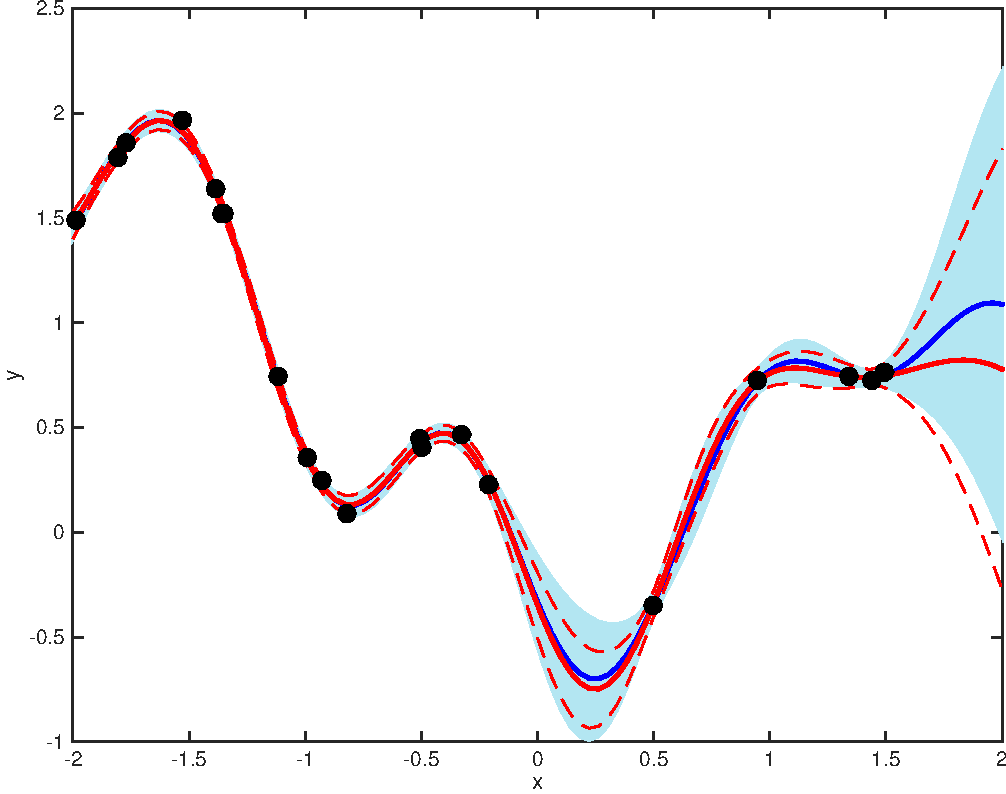
\includegraphics[width=0.45\textwidth]{alir}
\end{tabular}
\caption{Experiments on 1d input and 1000 features (bases). Left: using the 
``traditional FT convention". Right: Using Ali Rahimi's convention. 
The red curves are the mean and two standard errors of the predictive distribution by a GP.
The blue line and colored area are the same measures using  \rks. }
\end{figure}
\end{document}














